\documentclass[11pt,a4paper]{article}
\usepackage[margin=2.2cm]{geometry}
\usepackage[T1]{fontenc}\usepackage{lmodern}\usepackage{microtype}
\usepackage{xcolor,booktabs,tabularx,array,graphicx,float,enumitem,hyperref,fancyhdr,tikz,pgfplots}
\usetikzlibrary{arrows.meta,positioning,shapes.geometric,fit}
\pgfplotsset{compat=1.18}
\definecolor{navy}{HTML}{17324D}\definecolor{blue}{HTML}{277DA1}\definecolor{green}{HTML}{43AA8B}\definecolor{orange}{HTML}{F8961E}\definecolor{pale}{HTML}{EEF5F7}
\hypersetup{colorlinks=true,linkcolor=navy,urlcolor=blue}
\pagestyle{fancy}\setlength{\headheight}{14pt}\fancyhf{}\lhead{EC8203 Applied Big Data Engineering}\rhead{Smart Grid Pulse}\cfoot{\thepage}
\setlength{\parindent}{0pt}\setlength{\parskip}{5pt}\setlist{nosep,leftmargin=*}
\newcommand{\code}[1]{\texttt{#1}}
\begin{document}
\begin{titlepage}
\centering\vspace*{2.0cm}
{\color{blue}\large DATA ENGINEERING MINI-PROJECT\par}\vspace{0.8cm}
{\Huge\bfseries\color{navy} Smart Grid Pulse\par}\vspace{0.3cm}
{\Large A Kappa Pipeline for Live Grid Monitoring and Daily Billing\par}\vspace{1.4cm}
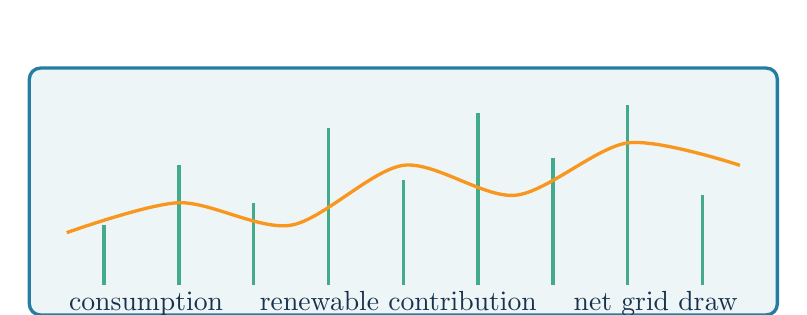
\begin{tikzpicture}[scale=.95]
\draw[fill=pale,draw=blue,very thick,rounded corners] (0,0) rectangle (10,3.3);
\foreach \x/\h in {1/1.2,2/2.0,3/1.5,4/2.5,5/1.8,6/2.7,7/2.1,8/2.8,9/1.6}{\draw[green,very thick] (\x,.4)--(\x,\h);}
\draw[orange,very thick,smooth] plot coordinates{(.5,1.1)(2,1.5)(3.5,1.2)(5,2.0)(6.5,1.6)(8,2.3)(9.5,2.0)};
\node[navy] at (5,.15) {consumption \quad renewable contribution \quad net grid draw};
\end{tikzpicture}
\vfill
\begin{tabular}{rl}
Module: & EC8203 - Big Data Analytics\\
Member 1: & Madakaladeniya I.U / EG/2021/4651\\
Member 2: & Wijesinghe S.A / EG/2021/4877\\
Submission date: & 30 September 2026\\
\end{tabular}
\vfill
\textit{One simulated day equals five minutes.}\par
\end{titlepage}

\tableofcontents\newpage

\section{Executive Summary}
Smart Grid Pulse is an end-to-end data platform answering two operational questions: what is the current grid load and renewable contribution in each zone, and what will each household owe after daily tariff data is applied? A Python producer generates meter readings every three seconds. Kafka provides a durable replayable log; Spark Structured Streaming cleans, deduplicates, derives net grid draw and produces one-minute zone metrics. A second Python source creates a daily tariff CSV. Apache Airflow runs this source every five minutes, publishes the records as reference events, upserts the current tariffs, and creates a daily household report. PostgreSQL supports the serving workload and FastAPI exposes live and daily results. JSON logs, Prometheus metrics, alert rules, Spark checkpoints and Airflow task history make system behaviour visible.

The design uses a Kappa architecture because the continuous event log is the authoritative history and both source types can be represented as immutable events. This eliminates two competing implementations of business rules. The submitted laptop deployment deliberately uses one broker and one Spark process for clarity and reproducibility; the report identifies the controls needed at production scale.

\section{Use Case and Requirements}
The selected scenario is Smart Grid Energy Monitoring and Billing. Twenty simulated households belong to four grid zones. Each meter emits consumption and solar generation values plus identity, zone and event time. Once per simulated day, the tariff provider drops a file describing rate, tier and subsidy status for every household.

The live output must report total consumption, solar generation, net imported energy, renewable percentage and active households for every zone. The daily output must join accumulated readings to the latest tariff and estimate each household's bill. The key non-functional requirements are replay after failure, duplicate protection, bounded handling of late events, transparent health signals, repeatable local setup and clear operator evidence.

\begin{table}[H]\centering\small
\caption{Requirement interpretation and acceptance evidence}
\begin{tabularx}{\textwidth}{>{\bfseries}p{.22\textwidth}X X}\toprule
Requirement & Implementation & Evidence \\\midrule
Streaming ingestion & Idempotent Kafka producer; household-keyed events every 3 s & Producer JSON logs and topic offsets\\
Daily source & Airflow creates one dated CSV each 5-minute simulated day & DAG run, CSV and task logs\\
Meaningful processing & Validation, deduplication, net-energy derivation and event-time windows & Spark job and PostgreSQL rows\\
Queryable output & Indexed PostgreSQL tables and FastAPI endpoints & Live and billing JSON responses\\
Observability & Structured logs, counters, latency histogram and two alert rules & Prometheus targets/rules and service logs\\
Reproducibility & Versioned images, Compose, schema initialization and tests & README commands and test results\\\bottomrule
\end{tabularx}\end{table}

\section{Architecture Decision: Kappa over Lambda}
\subsection{Decision drivers}
The dominant workload is a continuous append-only meter stream. Operators require seconds-to-minute freshness, deterministic recovery and a simple codebase that two students can explain. Daily tariff data changes reference state rather than requiring a separate historical computation engine. Kafka retention plus Spark checkpoints already provide replay, while PostgreSQL serves results without becoming the raw source of truth.

\subsection{Selected Kappa architecture}
All changes are events. Meter readings enter \code{meter-readings}; tariff rows enter \code{tariff-updates}, keyed by household. Spark processes the live stream and can recompute it from earlier offsets when logic changes. Airflow remains valuable: it owns the daily file boundary, publication, reference-table upsert and scheduled report. Kappa therefore describes the processing model, not the absence of orchestration or scheduled inputs.

\begin{figure}[H]\centering
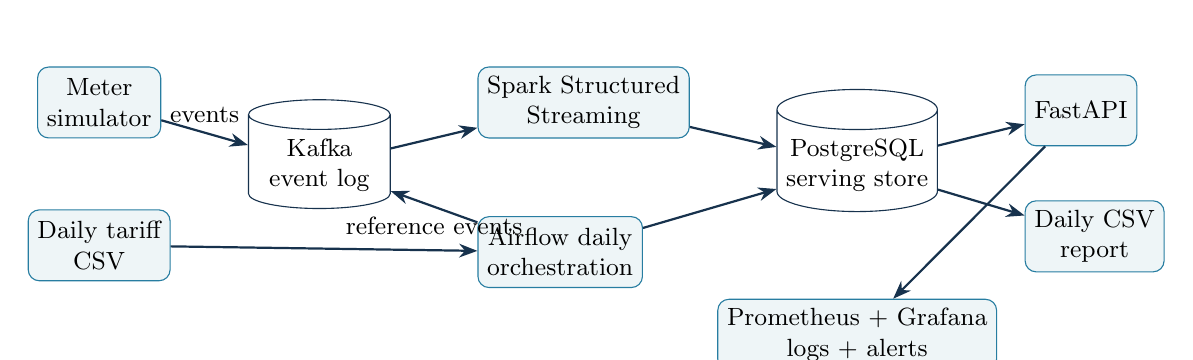
\begin{tikzpicture}[node distance=9mm and 11mm, every node/.style={font=\small}, box/.style={draw=blue,rounded corners,fill=pale,minimum height=9mm,align=center}, store/.style={draw=navy,cylinder,shape border rotate=90,aspect=.25,fill=white,minimum width=18mm,minimum height=12mm,align=center}, arr/.style={-{Stealth},thick,draw=navy}]
\node[box] (meter) {Meter\\simulator};
\node[box,below=of meter] (tariff) {Daily tariff\\CSV};
\node[store,right=of meter,yshift=-8mm] (kafka) {Kafka\\event log};
\node[box,right=of kafka,yshift=8mm] (spark) {Spark Structured\\Streaming};
\node[box,right=of kafka,yshift=-11mm] (airflow) {Airflow daily\\orchestration};
\node[store,right=of spark,yshift=-8mm] (pg) {PostgreSQL\\serving store};
\node[box,right=of pg,yshift=7mm] (api) {FastAPI};
\node[box,right=of pg,yshift=-9mm] (report) {Daily CSV\\report};
\node[box,below=of pg,yshift=-2mm] (obs) {Prometheus + Grafana\\logs + alerts};
\draw[arr] (meter)--node[above]{events}(kafka);\draw[arr] (tariff)--(airflow);\draw[arr] (airflow)--node[below]{reference events}(kafka);\draw[arr] (kafka)--(spark);\draw[arr] (spark)--(pg);\draw[arr] (airflow)--(pg);\draw[arr] (pg)--(api);\draw[arr] (pg)--(report);\draw[arr] (api)--(obs);
\end{tikzpicture}
\caption{Implemented Kappa-oriented architecture and control path}
\end{figure}

\subsection{Rejected Lambda alternative}
A Lambda design would preserve an immutable raw layer, run a historical batch path, and merge its views with a low-latency speed path. It can offer accurate recomputation and isolate late correction, but here it creates duplicate aggregation and joining logic, two consistency models and a serving-layer merge. Those costs are disproportionate for twenty simulated meters and one small daily reference file. Kappa has a single transformation path and replay mechanism. Its trade-off is that long replays may take time and schema evolution must remain compatible with retained events. Production mitigations include long Kafka retention or object-store archival, versioned schemas, shadow reprocessing topics and atomic view promotion.

\begin{table}[H]\centering\small
\caption{Architecture decision matrix (5 is best)}
\begin{tabular}{lcccl}\toprule Driver & Weight & Kappa & Lambda & Reason \\\midrule
Low latency & 25\% & 5 & 5 & Both support a speed path\\
Logic simplicity & 25\% & 5 & 2 & One versus two processing implementations\\
Replay/correction & 20\% & 4 & 5 & Kafka replay is sufficient at this scale\\
Cost/operations & 15\% & 5 & 2 & Fewer engines and views\\
Serving consistency & 15\% & 4 & 3 & No batch/speed merge race\\\midrule
Weighted score & & \textbf{4.65} & \textbf{3.55} & Kappa selected\\\bottomrule
\end{tabular}\end{table}

\section{Technology Stack and Rationale}
Kafka decouples producers from processing, partitions by household for ordered per-household history, and retains offsets for replay. A production topic would use at least three partitions and replication factor three; the Compose version uses a single broker to fit a student laptop. Idempotent producer mode reduces retry duplicates, while UUID event identifiers allow downstream deduplication.

Spark Structured Streaming was chosen over Storm because its DataFrame API expresses event-time windows, watermarks and PostgreSQL micro-batch writes concisely. Checkpoints persist offsets and progress. The two-minute watermark bounds state for delayed events. The \code{foreachBatch} sink makes SQL writes explicit, though production would stage each batch and merge transactionally for stronger exactly-once semantics.

Airflow models the daily boundary and exposes runs, dependencies, duration and failure. Its five-minute schedule compresses one day for demonstration. PostgreSQL provides constraints, indexes, joins and familiar query serving. FastAPI supplies typed discoverable endpoints and a Prometheus exposition endpoint. Prometheus evaluates availability and error-rate rules; Grafana provides the visualization surface. Docker Compose fixes component versions and networking for reproducibility.

\begin{table}[H]\centering\small
\caption{Major components and use-case-specific justification}
\begin{tabularx}{\textwidth}{p{.16\textwidth}p{.20\textwidth}X}\toprule Layer & Component & Why it fits \\\midrule
Ingestion & Kafka 7.6.1 & Back-pressure, household-key ordering, durable replay and independent consumers\\
Streaming & Spark 3.5.1 & Event-time windows, watermarking, schema parsing and scalable aggregations\\
Orchestration & Airflow 2.10.2 & Visible five-minute simulated-day schedule, retries and task evidence\\
Storage & PostgreSQL 16 & Relational tariff join, constraints, indexed latest-view queries and upserts\\
Serving & FastAPI & Lightweight live and daily JSON APIs plus generated OpenAPI documentation\\
Monitoring & Prometheus/Grafana & Numeric time-series, rule evaluation and operator dashboard foundation\\\bottomrule
\end{tabularx}\end{table}

\section{Data Ingestion and Processing}
The streaming generator emits twenty readings per cycle. Values are deliberately variable; solar is zero outside daylight hours. Each record includes an ISO-8601 UTC timestamp and UUID. Kafka keys preserve order for a household while allowing future partition parallelism. Structured JSON logs include the event and household identifiers so a demonstration can trace records.

Spark applies an explicit schema rather than inferring JSON, rejects missing identifiers and negative energy, parses event time, and calculates
\[
\textit{net\_grid\_kwh}=\max(0,\;\textit{consumption\_kwh}-\textit{solar\_generation\_kwh}).
\]
It deduplicates UUIDs and groups valid events into one-minute event-time windows by zone. Aggregates include consumption, solar, net grid draw, distinct active households and $100\times solar/consumption$. Records later than the two-minute watermark may be excluded from finalized windows; this is a stated freshness-versus-completeness choice.

The tariff generator writes twenty rows with lifeline, standard or peak rates. Publishing the rows to Kafka preserves the source change history; loading the same file into \code{tariffs} creates the serving snapshot. Airflow then joins daily readings to that snapshot and upserts \code{daily\_billing}. A rerun does not create duplicate bills because the key is report date plus household.

\section{Storage and Serving Design}
PostgreSQL separates atomic readings, time-window metrics, current tariffs and daily bills. A UUID primary key prevents duplicate meter events. Time/zone and latest-zone indexes match the main read patterns. Check constraints reject negative energy at the final boundary. The live endpoint uses \code{DISTINCT ON} with descending event time to return the newest window for every zone. The billing endpoint orders by estimated bill so high-cost households are immediately visible.

The daily charge is $net\ grid\ kWh \times tariff\ rate$. This is intentionally an estimate: export credits, taxes, standing charges and interval-specific prices are excluded. The API health endpoint executes a database query, so it detects dependency failure instead of only proving that the web process exists.

\section{Observability and Failure Handling}
Each Python stage emits JSON with time, severity, component and context. Kafka offsets and Spark checkpoint progress show whether consumption advances. Airflow records task state and duration for the scheduled path. FastAPI exports request counters and latency histograms. Prometheus scrapes every ten seconds.

Two rules meet and exceed the basic alert requirement. \textit{SmartGridApiDown} becomes critical when the API target is absent for one minute. \textit{SmartGridApiErrorRate} warns when server errors exceed 5\% for two minutes. In production, further rules would detect unchanged Kafka offsets, excessive consumer lag, missing daily files, stale zone metrics, checkpoint failures and reconciliation row-count differences.

Failure recovery is layered. Kafka buffers while Spark is unavailable; Spark resumes from its checkpoint. Producer idempotence reduces duplicates during retry, and event UUIDs stop duplicate storage. Airflow tasks can retry because tariff and report writes are upserts. PostgreSQL persistence resides in a named volume. Poison events are filtered in this version; production would send them to a dead-letter topic with validation reasons and alert on its rate.

\section{Results and Validation}
The repository includes a representative daily report. The three sample rows demonstrate different tariffs and renewable contributions. For H003, 18.420 kWh consumption minus 4.815 kWh solar yields 13.605 kWh net draw; at 0.31 currency units/kWh the rounded estimate is 4.22. H007 receives the lifeline rate and has a substantially smaller estimate.

\begin{table}[H]\centering\small
\caption{Representative consolidated daily output}
\begin{tabular}{l l r r r l r}\toprule Household & Zone & Use & Solar & Net grid & Tier & Bill \\\midrule
H003 & west & 18.420 & 4.815 & 13.605 & peak & 4.22\\
H007 & west & 12.160 & 5.230 & 6.930 & lifeline & 0.83\\
H010 & east & 15.780 & 8.620 & 7.160 & standard & 1.58\\\bottomrule
\end{tabular}\end{table}

\begin{figure}[H]\centering
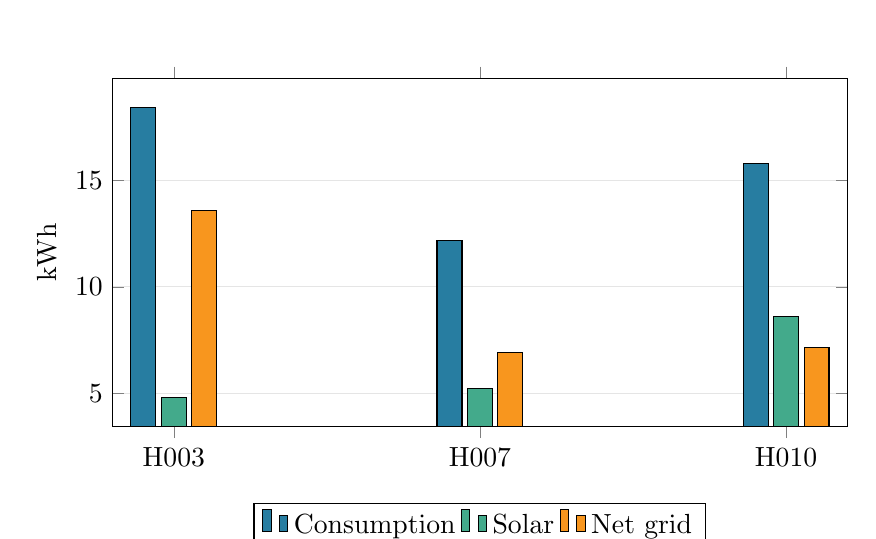
\begin{tikzpicture}
\begin{axis}[ybar,bar width=9pt,width=.9\textwidth,height=6cm,ylabel={kWh},symbolic x coords={H003,H007,H010},xtick=data,legend style={at={(.5,-.22)},anchor=north,legend columns=-1},ymajorgrids=true,grid style={gray!20}]
\addplot[fill=blue] coordinates {(H003,18.42)(H007,12.16)(H010,15.78)};
\addplot[fill=green] coordinates {(H003,4.815)(H007,5.23)(H010,8.62)};
\addplot[fill=orange] coordinates {(H003,13.605)(H007,6.93)(H010,7.16)};
\legend{Consumption,Solar,Net grid}
\end{axis}\end{tikzpicture}
\caption{Sample household energy reconciliation}
\end{figure}

Automated tests validate source fields, non-negative readings, all twenty tariff rows and the zero-floor net-grid formula. The demo smoke script checks health, live output and Prometheus exposition. Operational validation should also confirm all Compose services are healthy, Spark logs show completed batches, the Airflow DAG succeeds, a CSV appears, and Prometheus shows the API target as up.

\section{Security, Governance and Data Quality}
The local credentials are intentionally non-secret demonstration defaults and must never be reused. Production would place credentials in a secret manager, enable TLS and SASL for Kafka, use least-privilege service accounts, restrict network paths, rotate credentials and audit API access. A schema registry would enforce compatible meter and tariff evolution. Data-quality controls would include expected household coverage, tariff range checks, timestamp drift, physical bounds, duplicate ratios and reconciliation totals. Retention and deletion policies would be attached to raw events and household reports; the design avoids personal names and addresses but household identifiers remain potentially sensitive.

\section{Limitations and Production Evolution}
The single Kafka broker, local Spark process, SQLite-backed Airflow metadata and one PostgreSQL node provide no high availability. Random data does not reproduce spatial or seasonal correlation. Spark's append then aggregate writes are not a single cross-table transaction; a crash between them can create a temporarily inconsistent view. The reference event stream is published but the demonstration reconciliation deliberately reads the relational current snapshot. Grafana provisions a datasource, not a polished domain dashboard, because the assessed business outputs are the API and report.

At production scale we would deploy replicated Kafka with topic compaction for tariffs, Spark on Kubernetes with remote checkpoints, Airflow with PostgreSQL metadata and distributed workers, and managed PostgreSQL with partitioning and replicas. Raw events would also land in versioned Parquet on object storage to support inexpensive long-term replay. A schema registry, dead-letter topic, contract tests, OpenTelemetry traces and end-to-end freshness service-level objectives would strengthen governance and diagnosis. Billing would use interval tariffs, export credits and immutable tariff-effective periods rather than only the latest rate.

\section{Team Contributions and Delivery Plan}
The implementation is scoped for two members with balanced ownership and cross-review. Names and student IDs must replace the placeholders before submission.

\begin{table}[H]\centering\small
\caption{Two-person contribution statement}
\begin{tabularx}{\textwidth}{p{.24\textwidth}X X}\toprule & Primary implementation & Report/demo responsibility \\\midrule
Member 1 [Name/ID] & Meter simulator, Kafka, Spark transformations, checkpointing, tests & Architecture decision, processing narrative, Spark demonstration\\
Member 2 [Name/ID] & Tariff source, Airflow, PostgreSQL, API, Prometheus/Grafana, Compose & Stack rationale, observability/results, scheduled-report demonstration\\
Joint & Integration, code review, failure testing & Final editing, limitations, rehearsal; both defend all core logic\\\bottomrule
\end{tabularx}\end{table}

\section{Conclusion}
Smart Grid Pulse satisfies the brief with two simulated source modes, Kafka ingestion, meaningful event-time processing, an Airflow-orchestrated daily feed, queryable storage, live and consolidated outputs, structured logs, metrics and alerts. Kappa is the better architectural fit because replayable events and one transformation path meet the latency and consistency needs without Lambda's duplicate logic. The solution is deliberately honest about laptop-scale compromises while preserving a clear route to a resilient production platform.

\appendix
\section{Reproduction and Demo Checklist}
Copy \code{.env.example} to \code{.env}; run \code{docker compose up --build -d}; wait for health checks; enable and trigger \code{smart\_grid\_daily}; inspect API docs on port 8000, Airflow on 8080, Prometheus on 9090 and Grafana on 3000. Run \code{python scripts/demo\_check.py}. Show producer and Spark JSON logs, a successful Airflow graph, live zone results, the generated report and Prometheus rules. Use \code{docker compose down} after the demo. Full commands and troubleshooting assumptions are in the root README.

\section{Core Data Contracts}
Meter events contain \code{event\_id}, \code{meter\_id}, \code{household\_id}, consumption, solar generation, zone and timestamp. Tariff rows contain household, numeric rate, tier, subsidy flag and effective date. Live metrics contain window bounds, zone, consumption, solar, net draw, active households and renewable percentage. Daily billing contains report date, household, zone, energy totals, tariff attributes and rounded estimated bill.
\end{document}
